\documentclass[resume]{subfiles}


\begin{document}
\begin{multicols}{3}
\section{ADC / DAC}
\textbf{Petite puissance} :\\
\textbf{Haute vitesse} :\\
Operational amplifier:\\
\begin{minipage}{\linewidth}
	\centering
    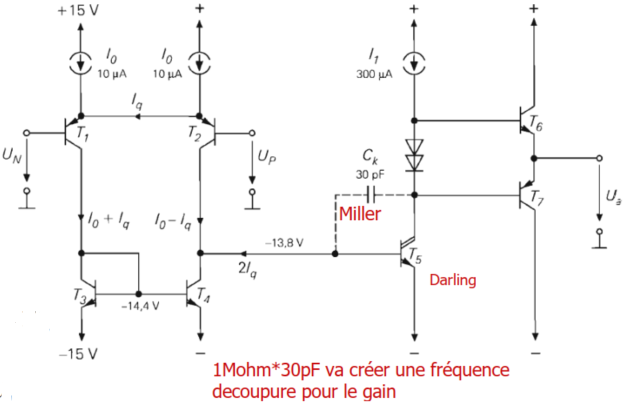
\includegraphics[width =0.7\columnwidth]{an17.png}
\end{minipage}\\
\begin{minipage}{\linewidth}
	\centering
    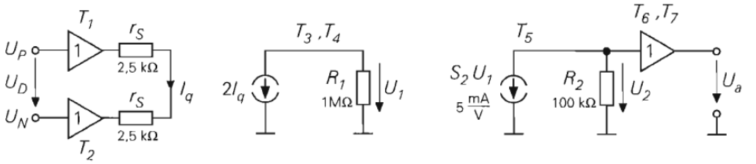
\includegraphics[width =0.7\columnwidth]{an18.png}
\end{minipage}\\
\begin{minipage}{\linewidth}
	\centering
    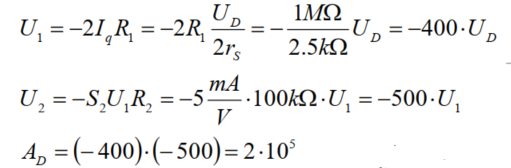
\includegraphics[width =0.7\columnwidth]{an19.png}
\end{minipage}\\
$f_0 = \frac{1}{2\pi R_1C_k}\cdot \frac{r_{s5}}{R_2}$\\
%%%%%%%%%%%%%%%%%%%%%%%%%%%%%%%%%
{\Large \textbf{ADC}}\\
\textbf{Quantization of the amplitude}
Resolution N is the number of bits \\
Resolution step is the analog value of the interval between two codes (1LSB)\\
$Code =\frac{V_{in}}{V_{FS}}\cdot (2^N-1)$\\
Quantification de l'erreur:\\
Power : $E_N=\frac{1}{V_{LSB}}\int_{-q/2}^{q/2}V_{ERR}^2(V_{iN})dV_{IN}=\frac{V_{LSB}^2}{12}$\\
$U_N=\frac{V_{LSB}}{\sqrt{12}}$\\
\begin{minipage}{\linewidth}
	\centering
    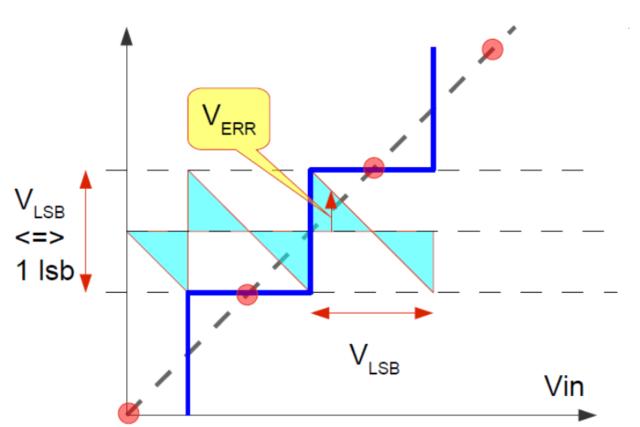
\includegraphics[width =0.7\columnwidth]{an1.png}
\end{minipage}\\
INL (Integral non linearity): différence entre la valeur actuelle et la valeur idéale\\
\begin{minipage}{\linewidth}
	\centering
    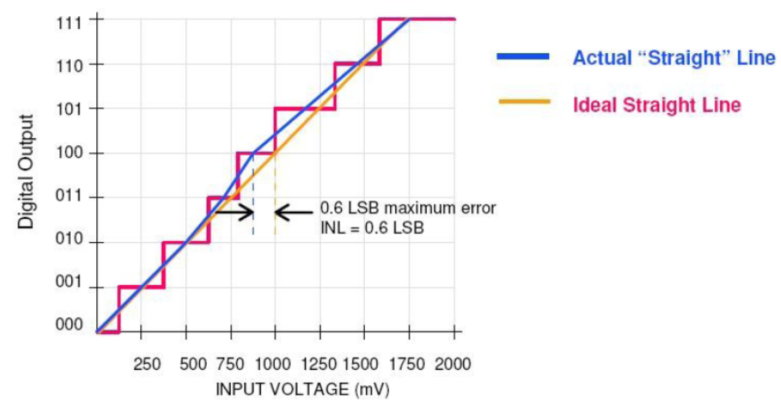
\includegraphics[width =0.7\columnwidth]{an2.png}
\end{minipage}\\
DNL : différence entre entre le step actuel et le step idéal\\
DNL > -1 : non monotonic\\
DNL > +1 : missing code\\
\begin{minipage}{\linewidth}
	\centering
    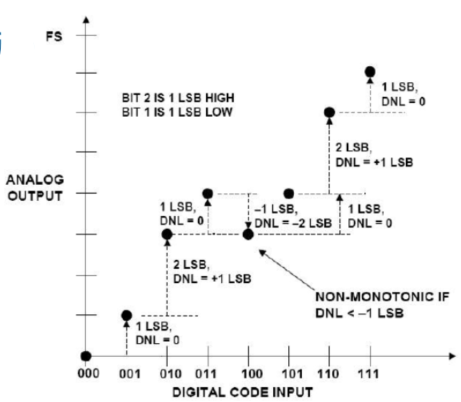
\includegraphics[width =0.7\columnwidth]{an3.png}
\end{minipage}\\
SNR(signal over noise power ratio):\\
$SNR_{dB}=10\cdot log(\frac{signal\ power\ P_S}{noise\ power\ P_N})$\\
$SNR_{dB}=20\cdot log(\frac{signal\ RMS\ voltage\ U_S}{noise\ RMS\ voltage\ U_N})$\\
THD (Total Harmonic distorsion): ratio entre deux valeurs RMS\\
$THD=\sqrt{\frac{\sum U_{h2}^2+U_{h3}^2+...+U_{hn}^2}{U_{Sin}^2}}$\\
(résultat entre 0 et 1)\\
SINAD (signal to noise and distorsion):\\
$SINAD=10\cdot log\frac{A_{SinFS}^2}{\sum (noise+distortion)power\ to\ fs/2}$
ENOB (Effective number of bits):\\
$ENOB=\frac{SINAD_{dB}-1.76}{6.02}$\\
Structure unary : série of $2^N$ times $2^0$ values\\
Resistor chain (kelvin divider)\\
\begin{minipage}{\linewidth}
	\centering
    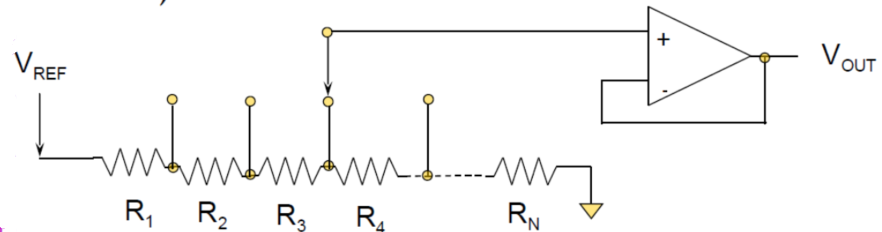
\includegraphics[width =0.7\columnwidth]{an4.png}
\end{minipage}\\
Segmented chains:\\
\begin{minipage}{\linewidth}
	\centering
    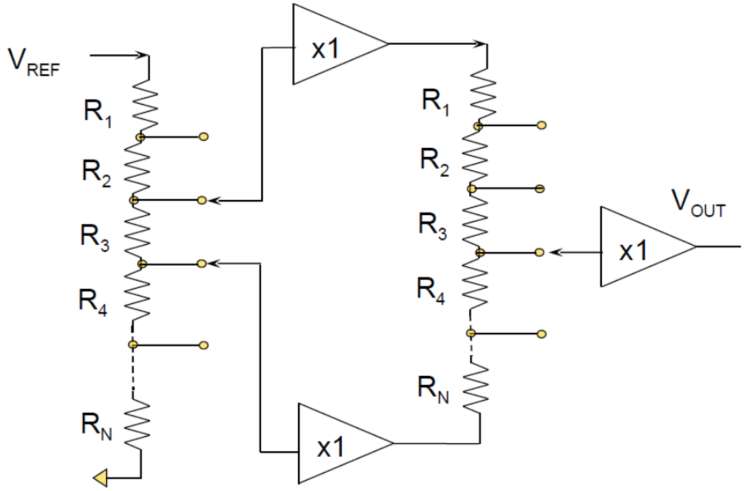
\includegraphics[width =0.7\columnwidth]{an5.png}
\end{minipage}\\
Structure binary : N different values($2^0,2^1,2^2,2^3...2^{N-1}$)\\
Binary-weighted structure\\
\begin{minipage}{\linewidth}
	\centering
    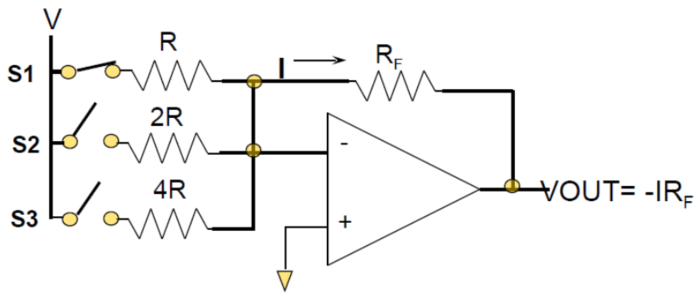
\includegraphics[width =0.7\columnwidth]{an6.png}
\end{minipage}\\
\begin{minipage}{\linewidth}
	\centering
    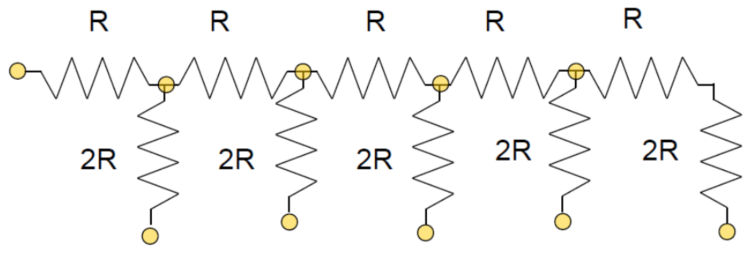
\includegraphics[width =0.7\columnwidth]{an7.png}
\end{minipage}\\
U-I output:\\
\begin{minipage}{\linewidth}
	\centering
    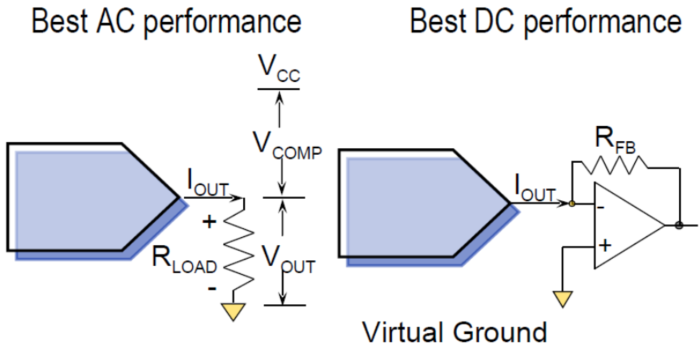
\includegraphics[width =0.7\columnwidth]{an8.png}
\end{minipage}\\
ADC structures : \\
\begin{minipage}{\linewidth}
	\centering
    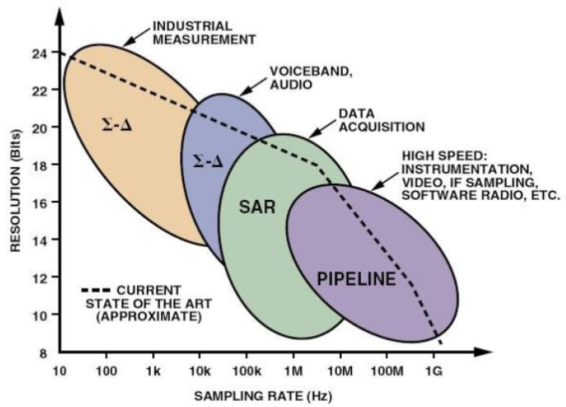
\includegraphics[width =0.7\columnwidth]{an9.png}
\end{minipage}\\
Flash converter: $2^N$ resistors and $2^N$ comparators. Speed between 100M and 1G sps. No S/H neeeded.\\
\begin{minipage}{\linewidth}
	\centering
    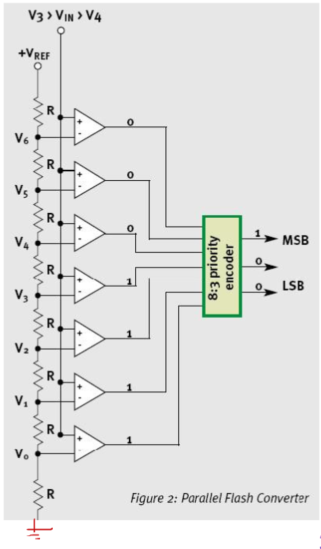
\includegraphics[width =0.7\columnwidth]{an10.png}
\end{minipage}\\
Pipeline converter: chaque étage représente un bit. Speed between 1M and 500M sps. S/H needed at each stage.\\
\begin{minipage}{\linewidth}
	\centering
    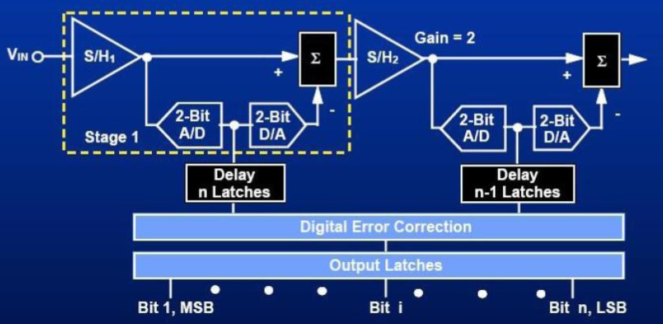
\includegraphics[width =0.7\columnwidth]{an11.png}
\end{minipage}\\
SAR converter: speed between 100k and 10M sps. Need S/H.\\
\begin{minipage}{\linewidth}
	\centering
    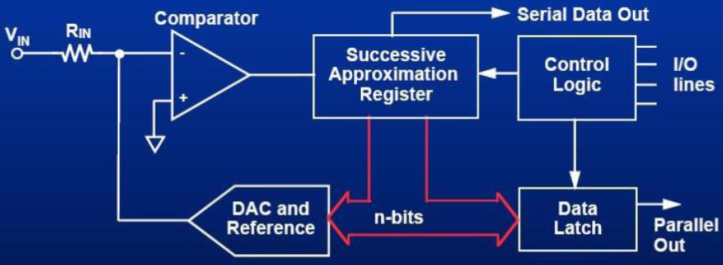
\includegraphics[width =0.7\columnwidth]{an12.png}
\end{minipage}\\
Noise sources:\\
\begin{itemize}
	\item quantization noise
	\item noise generated by the converter itself
	\item application circuit noise (reference \& power supply, GND bounce, layout considerations)
	\item Clock jitter (sampling)
\end{itemize}
\begin{minipage}{\linewidth}
	\centering
    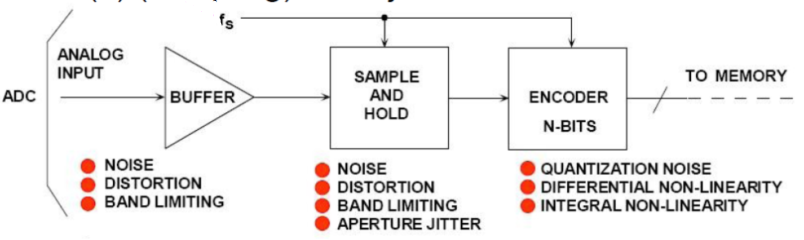
\includegraphics[width =0.7\columnwidth]{an13.png}
\end{minipage}\\
Analog input circuit noise is additive. Voltage reference noise is multiplicative. Quantisation noise is additive.\\
Single ended and common mode:\\
\begin{minipage}{\linewidth}
	\centering
    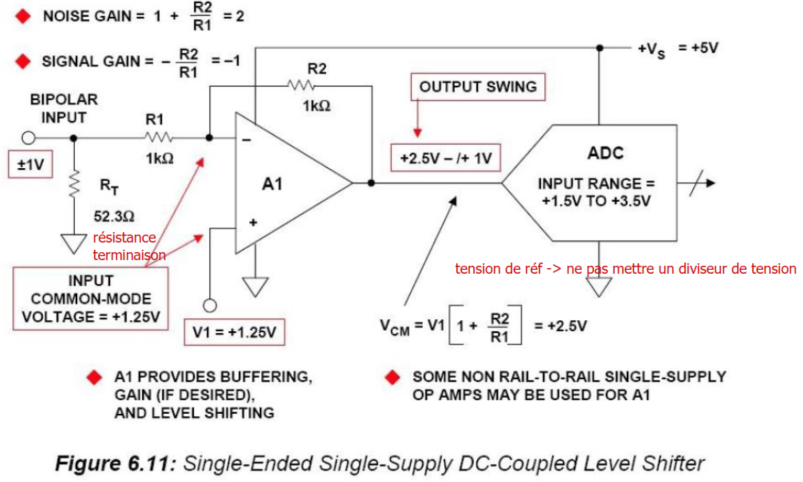
\includegraphics[width =0.7\columnwidth]{an14.png}
\end{minipage}\\
Single ended to differential (AC) conversion :\\
\begin{minipage}{\linewidth}
	\centering
    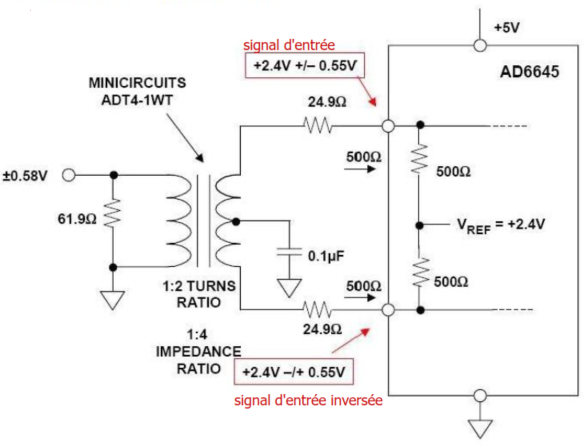
\includegraphics[width =0.7\columnwidth]{an15.png}
\end{minipage}\\
Single ended to differential (DC) conversion :\\
\begin{center}
	\centering
    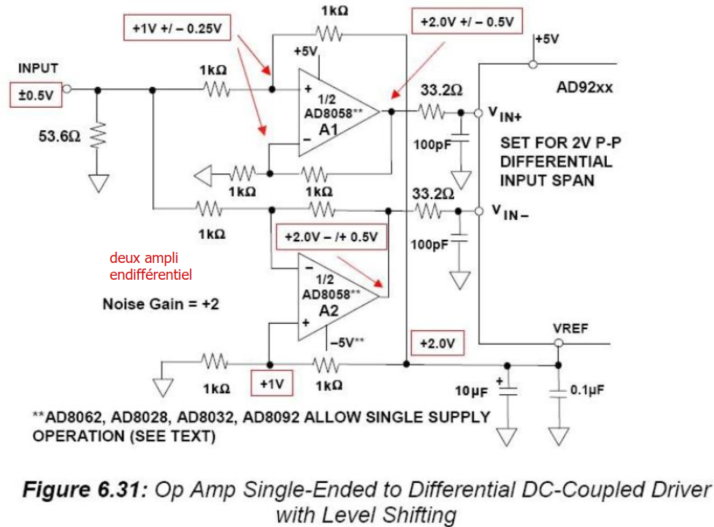
\includegraphics[width =0.7\columnwidth]{an16.png}
\end{center}
\subsection{Discrétisation}
Valeur du signal continu pris à des temps précis (sample)
Après l'échantillonnage, la valeur est quantifiée sur une valeur de $2^n$
\subsubsection{Idéal}
\begin{equation}
x_s(t) = \sum^{+\infty}_{k=-\infty} x(kT_s)\cdot \delta(t-kT_s) = x(t)\cdot \sum^{+\infty}_{k=-\infty} \delta(t-kT_s)
\end{equation}
\subsubsection{Critère de Nyquist}
$f_s > 2(f_a-f_b)$ avec $f_a$ limite haute de la BW du signal et $f_b$ limite basse de la BW

\subsection{Aliasing}
L'échantillonnage d'un signal provoque une répétition du spectre du signal autour de $f_s$ et de multiples de $f_s$.

\subsection{Signal Noise Ratio}
\begin{itemize}
\item Bruit de quantification RMS $N_{RMS} = \frac{V_{LSB}}{\sqrt{12}}$
\item Tension sinus FullScale $S_{RMS}\frac{V_{LSB}}{\sqrt{2}}\cdot \frac{2^N}{2}$
\item $SNR = 20log(\frac{S_{RMS}}{N_{RMS}}) = 20log(\sqrt{\frac{12}{8}}) + 20log(2^N)$
\item En dB $SNR = 6.02N + 1.76 $
\end{itemize}

\subsection{Process gain}
C'est lorsque l'on utilise pas toute la bande de 0 à $f_s/2$
le gain pour un sinus FullScale est le suivant.
\begin{equation}
SNR = 6.02N + 1.76 + 10log(\frac{f_s}{2\cdot BW})
\end{equation}

\subsection{Sur-échantillonnage}
\begin{equation}
SNR = 6.02N + 1.76 + 10log(OSR)
\end{equation}
Meilleur de 3dB à chaque fois que la $f_s$ double.

\subsection{Conversion Sigma-Delta}
\paragraph{Modulateur de premier ordre}
\subparagraph{Analogique}
\begin{figure}[H]
    \centering
    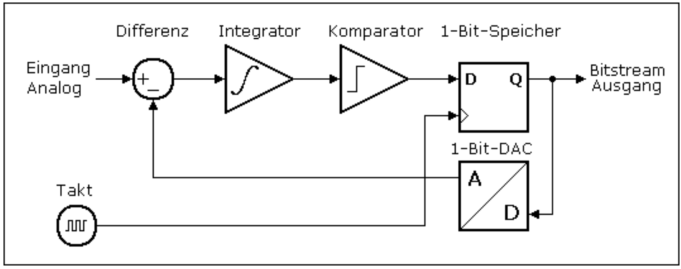
\includegraphics[width=0.8\columnwidth]{../images/OpAmp1/1ordreSD.png}
\end{figure}

\subparagraph{Digital}
\begin{figure}[H]
    \centering
    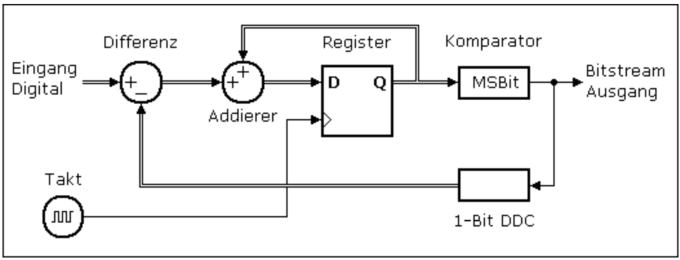
\includegraphics[width=0.8\columnwidth]{../images/OpAmp1/1ordreSDnum.png}
\end{figure}

\paragraph{Modulateur du deuxième ordre}
\begin{figure}[H]
    \centering
    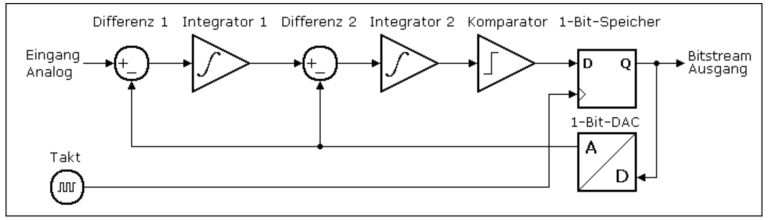
\includegraphics[width=0.8\columnwidth]{../images/OpAmp1/2ordreSD.png}
\end{figure}

\subsubsection{Sur-échantillonnage pour SD}
\begin{figure}[H]
    \centering
    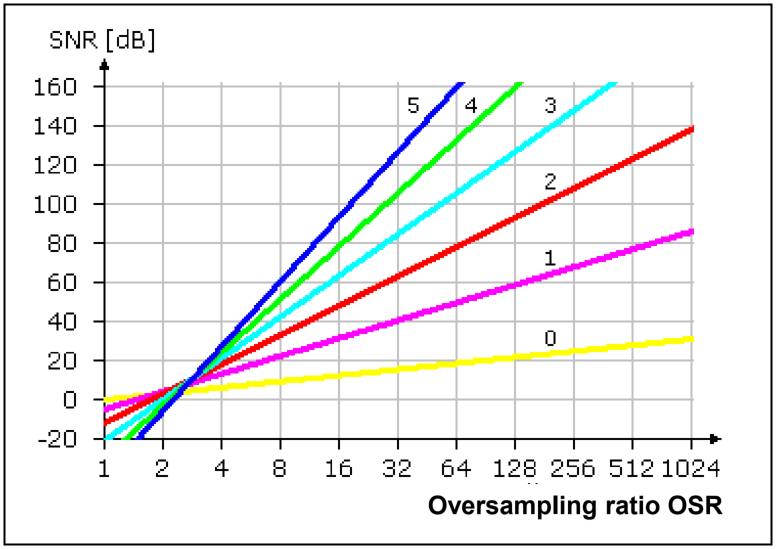
\includegraphics[width=0.8\columnwidth]{../images/OpAmp1/oversampling.png}
\end{figure}
\end{multicols}






\end{document}